% -----------------------------------------------
% chktex-file 44
\documentclass[../index.tex]{subfiles}

% -----------------------------------------------

\begin{document}

%- -----------------------------------------------
\renewcommand{\sectiontitle}{Let's talk about the web}
\section{\sectiontitle}
%- Without getting into much detail, let's get a brief high-level overview of what happens when
%- you go on a website in your web browser.
%-
%- Since this is meant to be pretty quick and more hands-on, we're going to totally skip network
%- stuff

%- ---------------------------
\renewcommand{\currenttitle}{\sectiontitle}
\begin{frame}[fragile]{\currenttitle}
%- Here's a pretty barebones diagram of a generic client-server architecture.
%-
%- The client process will send a request to the server, which is running a loop to listen for
%- requests.
%- When the server receives the request, it'll do some action and then return a response.
%- The client will be waiting for the response, and when it gets it, it'll maybe do something
%- based on that response.
%-
%- So you have this loop of client making requests and server returning responses.
%-
%- Remember that this is a rather generic pattern, so it can be applied to many things.
  \begin{figure}
    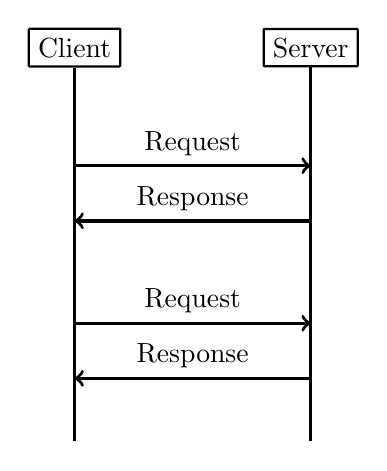
\begin{tikzpicture}[every node/.append style={thick,rounded corners=0.1mm}]
      \node[draw,rectangle] (Client) at (0,0) {Client};
      \node[draw,rectangle] (Server) at (3,0) {Server};

      \draw [very thick] (Client)--++(0,-5);
      \draw [very thick] (Server)--++(0,-5);

      \draw [->,very thick] (0,-1.5)--node [auto] {Request}++(3,0);
      \draw [<-,very thick] (0,-2.2)--node [auto] {Response}++(3,0);

      \draw [->,very thick] (0,-3.5)--node [auto] {Request}++(3,0);
      \draw [<-,very thick] (0,-4.2)--node [auto] {Response}++(3,0);
    \end{tikzpicture}
    \caption{Client-server communication}
  \end{figure}
\end{frame}

%- ---------------------------
\begin{frame}[fragile]{\currenttitle}
%- In our case, we're talking about the web, so let's make this diagram a little more specific.
%-
%- The modern web is dominated by a protocol known as HTTP. You've probably heard these letters
%- strung together before.
%- It stands for Hyper-Text Transfer Protocol.
%- This is the protocol the client and server use to send and receive requests and responses.
%-
%- So, the client, in our case, the web browser or some other web client, will send what we'll
%- call an HTTP request.
%- The server receives, it does something, and return a response.
%-
%- The technical specifics of HTTP or any other network protocol is way out of the scope of this
%- workshop, so we'll just leave it at that.
  \vspace*{1em}
  \textbf{HTTP} \textendash{} protocol used by most web clients and servers \\

  \vspace*{1em}
  \begin{figure}
    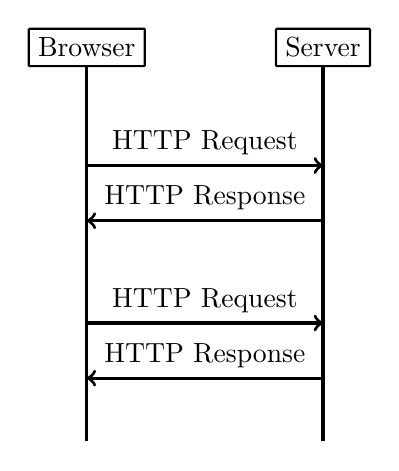
\begin{tikzpicture}[every node/.append style={thick,rounded corners=0.1mm}]
      \node[draw,rectangle] (Client) at (0,0) {Browser};
      \node[draw,rectangle] (Server) at (3,0) {Server};

      \draw [very thick] (Client)--++(0,-5);
      \draw [very thick] (Server)--++(0,-5);

      \draw [->,very thick] (0,-1.5)--node [auto] {HTTP Request} ++(3,0);
      \draw [<-,very thick] (0,-2.2)--node [auto] {HTTP Response}++(3,0);

      \draw [->,very thick] (0,-3.5)--node [auto] {HTTP Request} ++(3,0);
      \draw [<-,very thick] (0,-4.2)--node [auto] {HTTP Response}++(3,0);
    \end{tikzpicture}
    \caption{Client-server HTTP communication}
  \end{figure}
\end{frame}

%- ---------------------------
\renewcommand{\currenttitle}{HTTP request methods}
\begin{frame}{\currenttitle}
%- What you do need to know is that there are different types of HTTP requests.
%- We call these methods.
%-
%- The most common ones are outlined in this table: GET, POST, PUT, and DELETE.
  There are different types of HTTP requests: \\

  \begin{table}
    \begin{tabular}{l l p{0.65\textwidth}} \hline
      \textbf{Method} & \textbf{Payload} & \textbf{Description} \\ \hline
      GET             & No               & Request some resource. \\
      POST            & Yes              & Create some resource, usually resulting in a state change. \\
      PUT             & Yes              & Update some resource. \\
      DELETE          & No               & Delete some resource. \\ \hline
    \end{tabular}
    \caption{HTTP request methods}
  \end{table}
\end{frame}

%- ---------------------------
\tikzset{req/.style={draw,rectangle split, rectangle split parts=2,align=left}}
\newcommand{\reqproperty}[2][\dots]{{\small #2: \texttt{#1}}}
\newcommand{\responsenode}[1]{%-
  \node [req]
    (#1) at (4,-1.5) {
      \textbf{HTTP Response}
      \nodepart{second}
      \reqproperty{Header} \\
      \reqproperty[200/400/\dots]{Code} \\
      \reqproperty{Body}
    }%-
}
\renewcommand{\currenttitle}{GET request}
\begin{frame}[fragile]{\currenttitle}
%- The GET request is pretty much what it sounds like: a request to get the value
%- of something.
%- We'll use the term 'resource' to generically refer to 'something'.
%-
%- We can't just make any old arbitrary request.
%- The server has to have defined and is listening on an 'endpoint' where we can make a certain
%- request.
%-
%- The endpoint is an ordinary URL like the ones you input into the address bar.
%- So, an endpoint might be something like api.duckduckgo.com/v1.
%-
%- Let's look at this diagram.
%-
%- The client sends a GET request to the specific endpoint on the server.
%- We'll pretend that /endpoint is the URL for that endpoint.
%-
%- The request will contain metadata in header values.
%- If this endpoint requires the client to be logged in or something, the headers might contain
%- an authentication token string.
%-
%- The server will receive and execute specific logic for that endpoint.
%- Then it'll return a response back to the client, which will contain header values of its own.
%-
%- One of the most important bits of information is the status code.
%- The HTTP spec defines codes such as 200, 201, 304, 401, 404, 500, etc. that the response
%- should contain.
%- These indicate to the client different things, usually regarding the success of the request.
%- For example, 200 tells the client that the request was a success.
%- 401 is an authentication error; it tells the client that the client is not authorized to access
%- this resource.
%-
%- And for GET requests, the response will contain data in the 'body'. This can come in whatever
%- format the server likes.
%- In modern web APIs, it's usually JSON (JavaScript Object Notation).
%-
%- If we have an API that gives access to information about films, a GET endpoint might return
%- data about a certain film.
  \vspace*{2em}

  \begin{figure}
    \begin{tikzpicture}[every node/.append style={thick,rounded corners=0.1mm,outer sep=1mm}]
      \node [draw,rectangle] (Client) at (0,0) {Client};
      \node [draw,rectangle] (Server) at (8,0) {Server};
      \node [req]
        (Request) at (4,1.5) {
          \textbf{GET} \texttt{/endpoint}
          \nodepart{second}
          \reqproperty{Header} \\
          \reqproperty{User Agent} \\
          \reqproperty[<empty>]{Body}
        };
      \draw [very thick] (Client)  to[out=90,in=180] (Request);
      \draw [->,very thick] (Request) to[out=0,in=90]   (Server);

      \responsenode{Response};
      \draw [very thick]    (Server)   to[out=270,in=0]   (Response);
      \draw [->,very thick] (Response) to[out=180,in=270] (Client);
    \end{tikzpicture}
    \caption{GET request}
  \end{figure}

\end{frame}

%- ---------------------------
\renewcommand{\currenttitle}{POST request}
\begin{frame}[fragile]{\currenttitle}
%- The POST request is typically made when you create something in the server.
%-
%- Let's say your server maintains a database of users.
%- A POST request might cause the backend to create a user with the specified properties.
%- That's a state change; the state of our database is now different than what it was before.
%-
%- Where do we specify those properties? In the request body.
%- So the request can also have a body just like the response.
%- Going with the user example, we might specify the username, email address, and other things
%- in the request body.
%-
%- When the server receives the request, it'll execute it's own logic to do whatever needs
%- to be done for that endpoint, and then return a response.
%-
%- It's similar for PUT and DELETE.
%- PUT requests usually also contain a body that tell the server what values to update with.
%- We'll just skip them for now.
%-
%- It's important to note that these methods are specifications that give clients expectations.
%- Your code will still compile if your DELETE endpoint functions like a GET request, but it
%- would confusing and not up to spec.
%-
%- If a server provides a GET endpoint, and I make a GET request there, I expect
%- to get back a resource.
%- I would not expect the server to modify or delete any resource.
%- That would be an erroneous implementation on the server side.
  \vspace*{2em}

  \begin{figure}
    \begin{tikzpicture}[every node/.append style={thick,rounded corners=0.1mm,outer sep=1mm}]
      \node [draw,rectangle] (Client) at (0,0) {Client};
      \node [draw,rectangle] (Server) at (8,0) {Server};
      \node [req]
        (Request) at (4,1.5) {
          \textbf{POST} \texttt{/endpoint}
          \nodepart{second}
          \reqproperty{Header} \\
          \reqproperty{User Agent} \\
          \reqproperty{Body}
        };
      \draw [very thick] (Client)  to[out=90,in=180] (Request);
      \draw [->,very thick] (Request) to[out=0,in=90]   (Server);

      \responsenode{Response};
      \draw [very thick]    (Server)   to[out=270,in=0]   (Response);
      \draw [->,very thick] (Response) to[out=180,in=270] (Client);
    \end{tikzpicture}
    \caption{POST request}
  \end{figure}
\end{frame}


% -----------------------------------------------

\end{document}
